\chapter{Introducci\'{o}n}
\textit{Staphylococcus aureus} es una bacteria pat\'{o}gena Gram Positiva que causa enfermedades infecciosas. De acuerdo a Kobayashi et al. \cite{Kobayashi2015PathogenesisAbscesses}, la bacteria es un colonizador com\'{u}n de la piel y del aparato respiratorio y act\'{u}a como un pat\'{o}geno oportunista que puede causar infecciones nicosomiales (intrahospitalarias) en el sistema respiratorio, en los tejidos blandos y en el torrente sangu\'ineo \cite{HarpavatS.NissimS.LipppincottsMicrocards:MicrobiologyFlashCards2012.}. Incluso puede causar infecciones en las junturas de las pr\'otesis formando biopel\'iculas \cite{Meylan2018}.\\

%En la figura \ref{fig:sta} se muestra una microfotograf\'ia de \textit{Staphylococcus aureus} resistente a antibi\'oticos.\\

%\begin{figure}[h]
%\begin{center}
 % 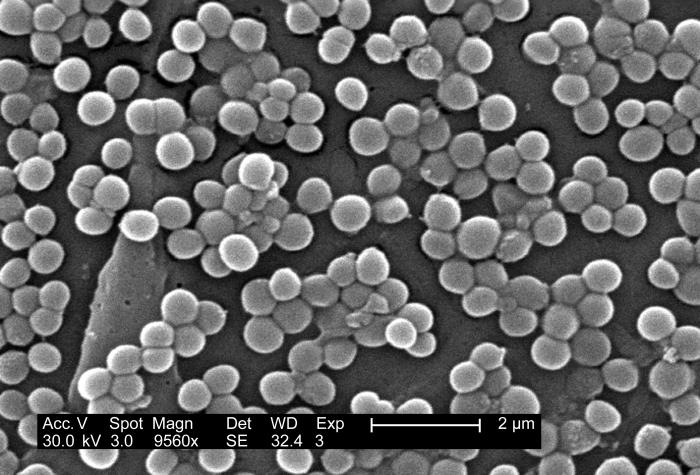
\includegraphics[scale=0.3]{saureus.jpg}
  %\caption{Imagen  de \textit{Staphylococcus aureus} obtenida con un microscopio electr\'onico de barrido (SEM). Tomado de \cite{HaneyCar2005PublicAureus}.}
  %\label{fig:sta}
%\end{center}
%\end{figure}

Desde el descubrimiento de \textit{Staphylococcus aureus} como causante de una infecci\'on a una herida en 1881 \cite{Orent2006AMagazine} se ha investigado su presencia en otras infecciones y se han utilizado antibi\'oticos como la penicilina, la meticilina y la vancomicina para controlar estas infecciones   \cite{HarpavatS.NissimS.LipppincottsMicrocards:MicrobiologyFlashCards2012.}. No obstante, \textit{Staphylococcus aureus} ha desarrollado resistencia a algunos de estos antibi\'oticos,  de ah\'{i} que surja la necesidad de buscar nuevos antibi\'oticos o incluso mol\'{e}culas con un mecanismo de acci\'{o}n diferente. Una posible familia de mol\'{e}culas que podr\'{i}an actuar como alternativas ser\'{i}an los p\'{e}ptidos antimicrobianos.\\

De acuerdo a Perez-Lopez et al. \cite{Perez-LopezVariationsProperties} y Nagendra et al.  \cite{Nagendra2011} se ha encontrado que la bacteria modula la composici\'{o}n de su membrana plasm\'{a}tica frente a cambios en el medio. Esta modulaci\'{o}n afecta las propiedades biof\'{i}sicas de su membrana, es decir propiedades fisicoqu\'{i}micas como la permeabilidad, la estructura y las propiedades mec\'{a}nicas. El cambio de estas propiedades es un factor que mejora la tolerancia de la bacteria a la acci\'{o}n de p\'{e}ptidos antimicrobiales. Debido a esto, las propiedades biof\'{i}sicas de la membrana se convierten en objeto de estudio y adem\'{a}s son determinantes en la b\'{u}squeda de nuevas mol\'{e}culas dirigidas a la membrana (mol\'{e}culas blanco) que combatan la bacteria. \\

Al ser \textit{Staphylococcus aureus}\footnote{\textit{Staphylococcus aureus} al ser una bacteria Gram positiva est\'{a} envuelta por una  membrana llamada bicapa lip\'{i}dica y recubierta de una pared externa de p\'{e}ptidoglicando. Las membranas se explican en la subsecci\'{o}n \ref{ss:mem}} una bacteria Gram positiva, consta de una membrana plasm\'{a}tica que es de inter\'{e}s en t\'{e}rminos de la generaci\'{o}n de nuevos antibi\'{o}ticos antimicrobiales debido a su rol como mediador del potencial electroqu\'{i}mico. Algunos estudios se han enfocado en c\'{o}mo la composici\'{o}n de la bicapa lip\'{i}dica interna afecta sus propiedades biof\'{i}sicas con base en cambios en la concentraci\'{o}n de ciertos l\'{i}pidos como la cardiolipina \cite{Hernandez-Villa1BiophysicalPeptides} y de carotenoides como la estafiloxantina \cite{MelendezDelgado2018StudyingBilayers}, \cite{Perez-LopezVariationsProperties}, \cite{Nagendra2011}. Recientemente, en nuestros grupos, se han estudiado computacionalmente y experimentalmente propiedades mec\'{a}nicas como la rigidez de la membrana, la orientaci\'{o}n de la estafiloxantina, el \'{a}rea por l\'{i}pido, la difusi\'{o}n y el par\'{a}metro de orden del deuterio de diferentes membranas modelo.\\

En los experimentos realizados por Perez-Lopez et al. \cite{Perez-LopezVariationsProperties} y Nagendra et al.  \cite{Nagendra2011} se ha mostrado que cambios en el contenido de carotenoides en las membranas, en diferentes etapas de crecimiento \textit{Staphylococcus aureus}, y en membranas modelo compuestas por algunos l\'{i}pidos mayoritarios de la bacteria, resultan en cambios en la rigidez. Se ha demostrado que este cambio en rigidez afecta la resistencia de la membrana a diferentes p\'{e}ptidos antimicrobiales. Sin embargo, es necesario mirar a nivel molecular la influencia local que tienen los carotenoides en la membrana para entender como la presencia de estas mol\'{e}culas puede influir en las propiedades mec\'{a}nicas. Debido a su resoluci\'{o}n, los experimentos realizados no permiten vislumbrar diferentes propiedades moleculares que puedan explicar este fen\'{o}meno. Alternativamente, las simulaciones de din\'{a}mica molecular (MD por sus siglas en ingl\'{e}s) si permiten hacer este acercamiento. La MD se ha convertido en una herramienta excelente para estudiar membranas biol\'{o}gicas \cite{Marrink2019ComputationalMembranes}. Este m\'{e}todo monitorea la evoluci\'{o}n espacio-temporal de sistemas biol\'{o}gicos a una escala at\'{o}mica y asi permite determinar informaci\'{o}n estructural (termo)din\'{a}mica y energ\'{e}tica de membranas, que complementa y expande las t\'{e}cnicas experimentales. 
Entre las propiedades que se pueden estudiar en detalle a trav\'{e}s de simulaciones est\'{a}n la ubicaci\'{o}n relativa de los carotenoides con respecto a los otros l\'{i}pidos, la orientaci\'{o}n y las interacciones que presenta exclusivamente el carotenoide estafiloxantina con los l\'{i}pidos vecinos. Estos detalles moleculares influyen en los cambios de la rigidez de la membrana de \textit{Staphylococcus aureus}.\\

Para estudiar la ubicaci\'{o}n, las interacciones con otros l\'{i}pidos, el \'{a}rea por l\'{i}pido,  de la estafiloxantina, en nuestro grupo se ha realizado un estudio computacional preeliminar mediante las simulaciones por din\'{a}mica molecular  implementadas en CHARMM \cite{MelendezDelgado2018StudyingBilayers}. Estas simulaciones requieren introducir ciertos par\'{a}metros relacionados con los campos de fuerza y con la geometr\'{i}a de la estafiloxantina, los cuales deben ser cuidadosamente seleccionados para que las simulaciones por din\'{a}mica molecular reflejen el comportamiento f\'{i}sico de la mol\'{e}cula.\\

En una aproximaci\'{o}n inicial, Mel\'{e}ndez et al. \cite{MelendezDelgado2018StudyingBilayers} utilizaron el protocolo implementado en CHARMM-GUI \cite{Sunhwan2008CHARMM-GUI:CHARMM} para determinar los par\'{a}metros de estafiloxantina. Algunos de los par\'{a}metros obtenidos a trav\'{e}s de este procedimiento para la estafiloxantina no se han optimizado completamente. El objetivo de la  presente propuesta es optimizar los par\'{a}metros generados por CHARMM-GUI para la estafiloxantina, para que luego puedan ser utilizados en simulaciones MD a la luz del trabajo previo realizado \cite{MelendezDelgado2018StudyingBilayers}. Adicionalmente, proponemos modelar la estafiloxantina utilizando un segundo campo de fuerzas (llamado AMBER). \'{e}ste modelamiento nos permitir\'{a} estudiar la din\'{a}mica de bicapas lip\'{i}dicas en presencia de estafiloxantina y confirmar que las observaciones que hagamos sean independientes del potencial de fuerzas utilizado.\\